\section{Problem Statement}\label{sec:problem-presentation}
For this work, three different functions are chosen to be numerically integrated. These functions are presented in this section, along with their analytical solutions. To integrate the functions the Trapezoidal, the Simpson's 1/3 and 3/8, and the Gauss-Legendre rules are employed. The results obtained by these methods are compared with the analytical solutions, and the error convergence is analyzed.

For every function, one presents the function itself and the analytical solution for the integral. A code in Mathematica is developed to help with the visualization.

\subsection{Function 1}
Function 1 is represented by Eq. \eqref{eq:func1} 
\begin{equation}
    \label{eq:func1}
    f(x) = e^{-\frac{(x-1)^2}{\epsilon}} \quad \forall x \in \mathbb{R} | 0 \leq x \leq 2, \epsilon\rightarrow 0,
\end{equation}
since it depends on the parameter $\epsilon$, a simple analysis over its behaviour its made. Fig. \ref{fig:func1} shows how it is the variation of the function for differente values of $\epsilon$.
\begin{figure}[H]
    \centering
    \subfloat[$\epsilon = 10^{-1}$]{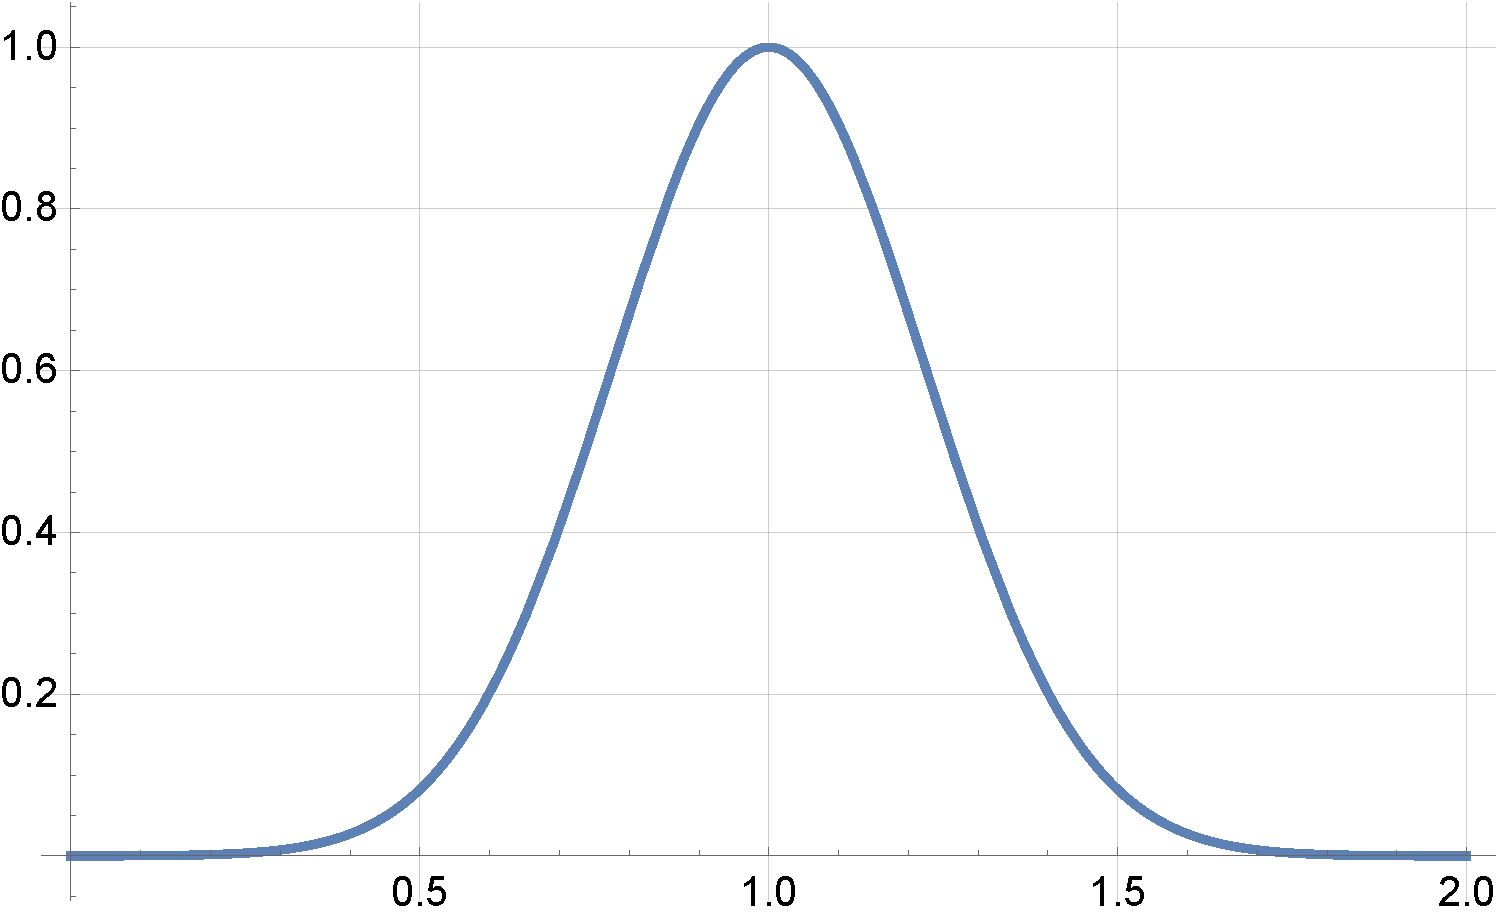
\includegraphics[width=0.5\textwidth]{../Figures/func1_e1.pdf}}\hfill
    \subfloat[$\epsilon=10^{-2}$]{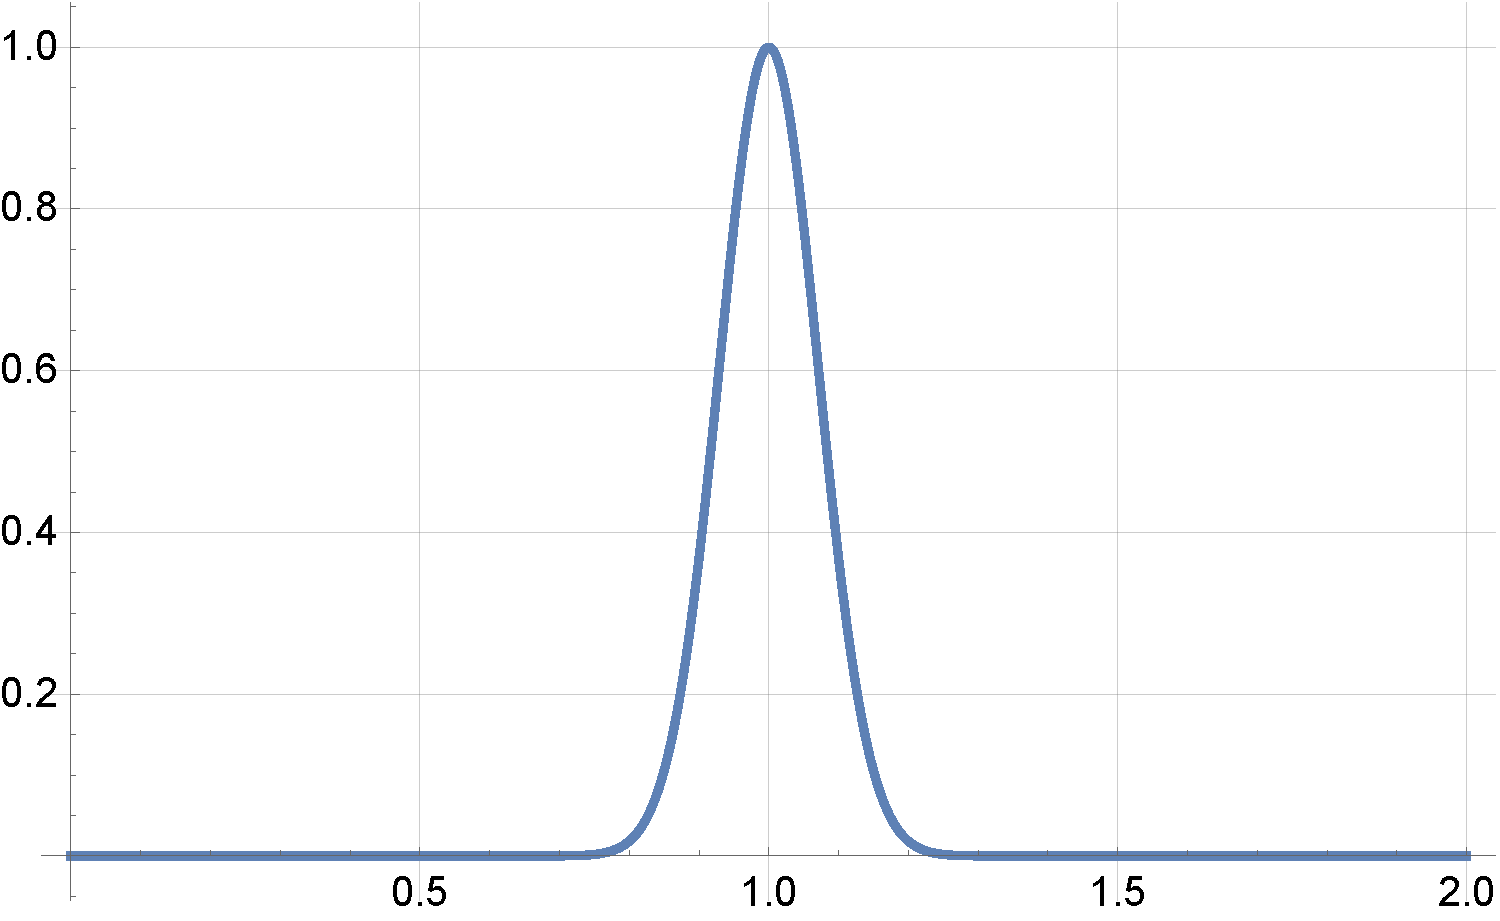
\includegraphics[width=0.5\textwidth]{../Figures/func1_e2.pdf}}\\
    \subfloat[$\epsilon=10^{-3}$]{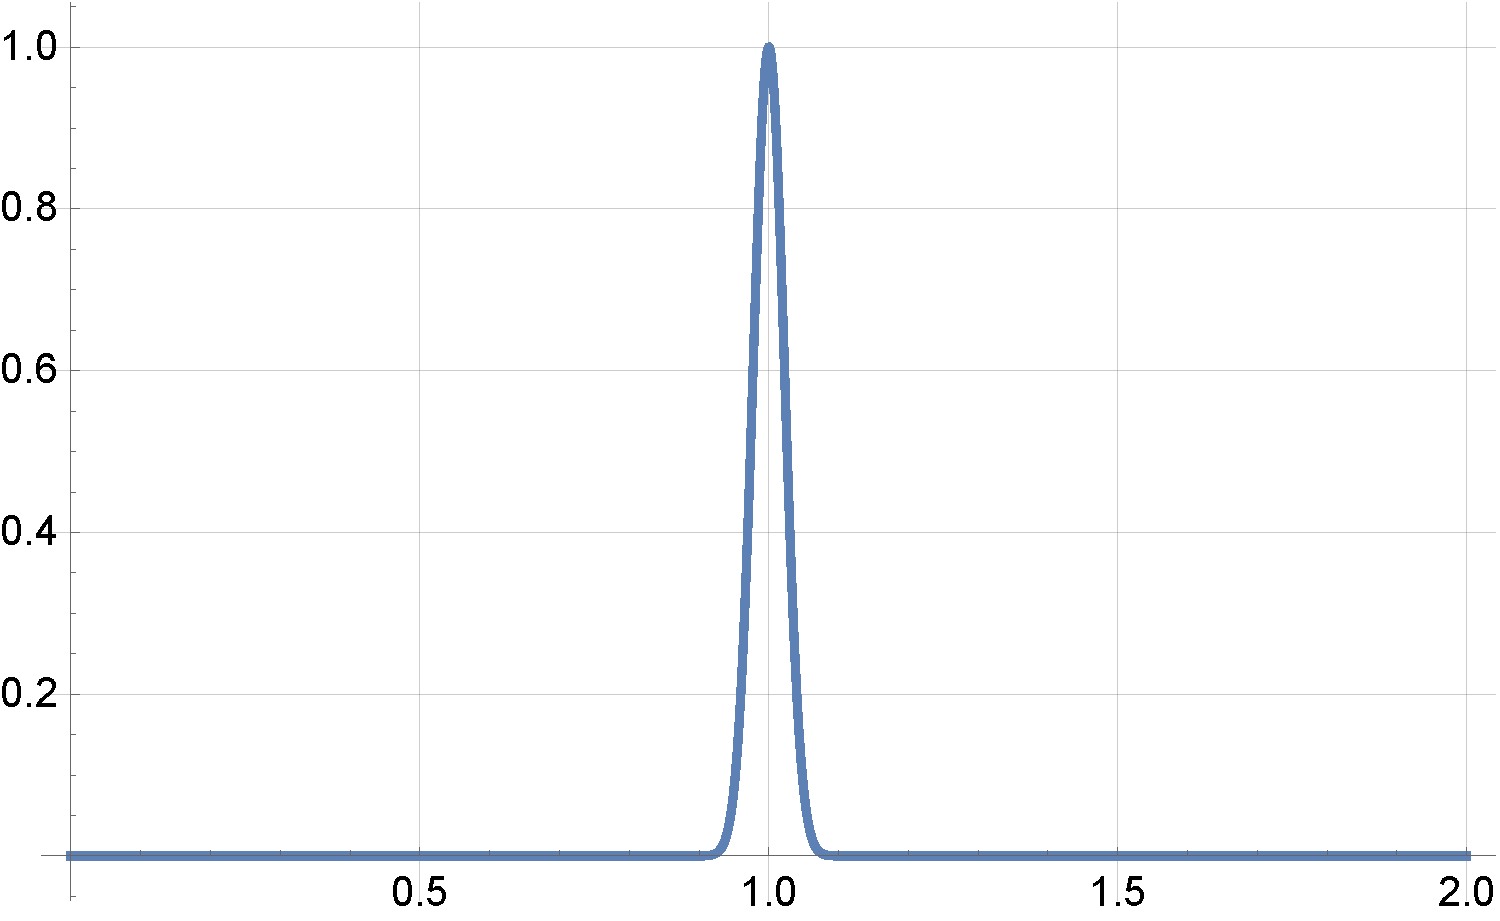
\includegraphics[width=0.5\textwidth]{../Figures/func1_e3.pdf}}\hfill
    \subfloat[$\epsilon=10^{-4}$]{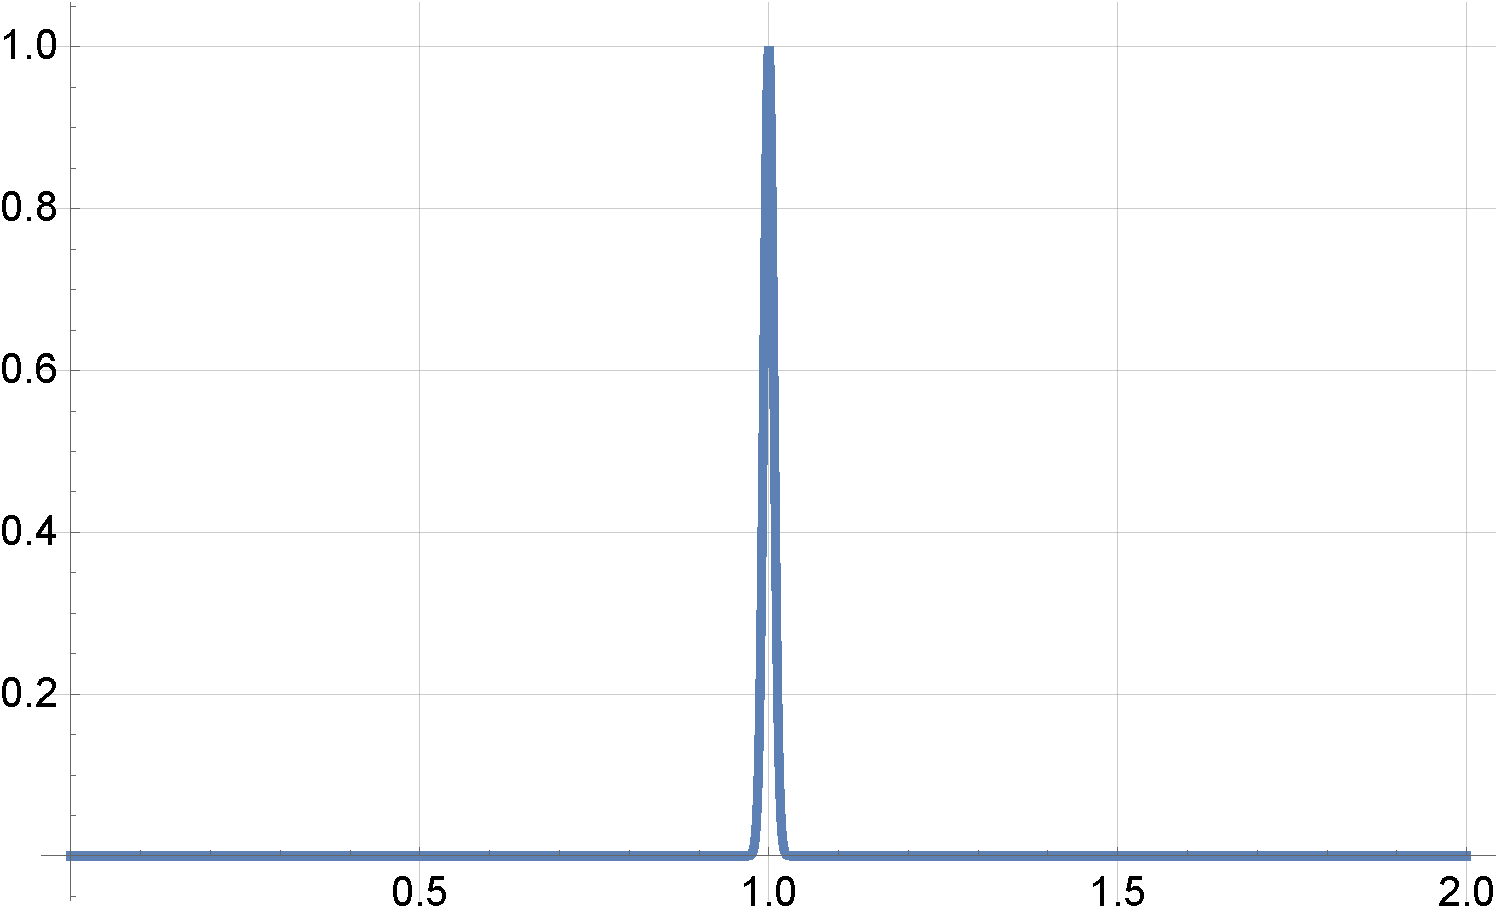
\includegraphics[width=0.5\textwidth]{../Figures/func1_e4.pdf}}
    \caption{Function 1}
    \label{fig:func1}
\end{figure}

By analyzing Fig. \ref{fig:func1}, one can note that, the lesser the value of $\epsilon$, the more the function behaves like a Dirac Delta function, which is not integrable. The analytical solution for the integral of the function is given by Eq. \eqref{eq:func1_integral}
\begin{equation}
    \label{eq:func1_integral}
    \int e^{-\frac{(x-1)^2}{\epsilon}} ~dx= \frac{\sqrt{\pi} ~\text{Erf}\left(c (- 1 + x)\right)}{2 c},
\end{equation}
in which c is a constant given by $c = pot\sqrt{10}$, and $pot$ is a integer number found in $\epsilon = 10^{-pot}$. Erf is the error function, defined by Eq. \eqref{eq:error_function}
\begin{equation}
    \label{eq:error_function}
    \text{Erf}(z) = \frac{2}{\sqrt{\pi}} \sum_{n=0}^{\infty} \frac{z}{2n + 1} \prod_{k=0}^{n} \frac{-z^2}{k}.
\end{equation}

In this work, the error function is evaluated using the Python library \texttt{scipy} and Function 1 is integrated considering two cases: $\epsilon = 1$ and $\epsilon = 10^{-4}$.
\subsection{Function 2}
Function 2 is given by Eq. \eqref{eq:func2} and Fig. \ref{fig:func2} shows its behaviour
\begin{equation}
    \label{eq:func2}
    f(x) = x\sin\left(\frac{1}{x}\right) \quad \forall x \in \mathbb{R} | 1/100 \leq x \leq 1/10.
\end{equation}
\begin{figure}[H]
    \centering
    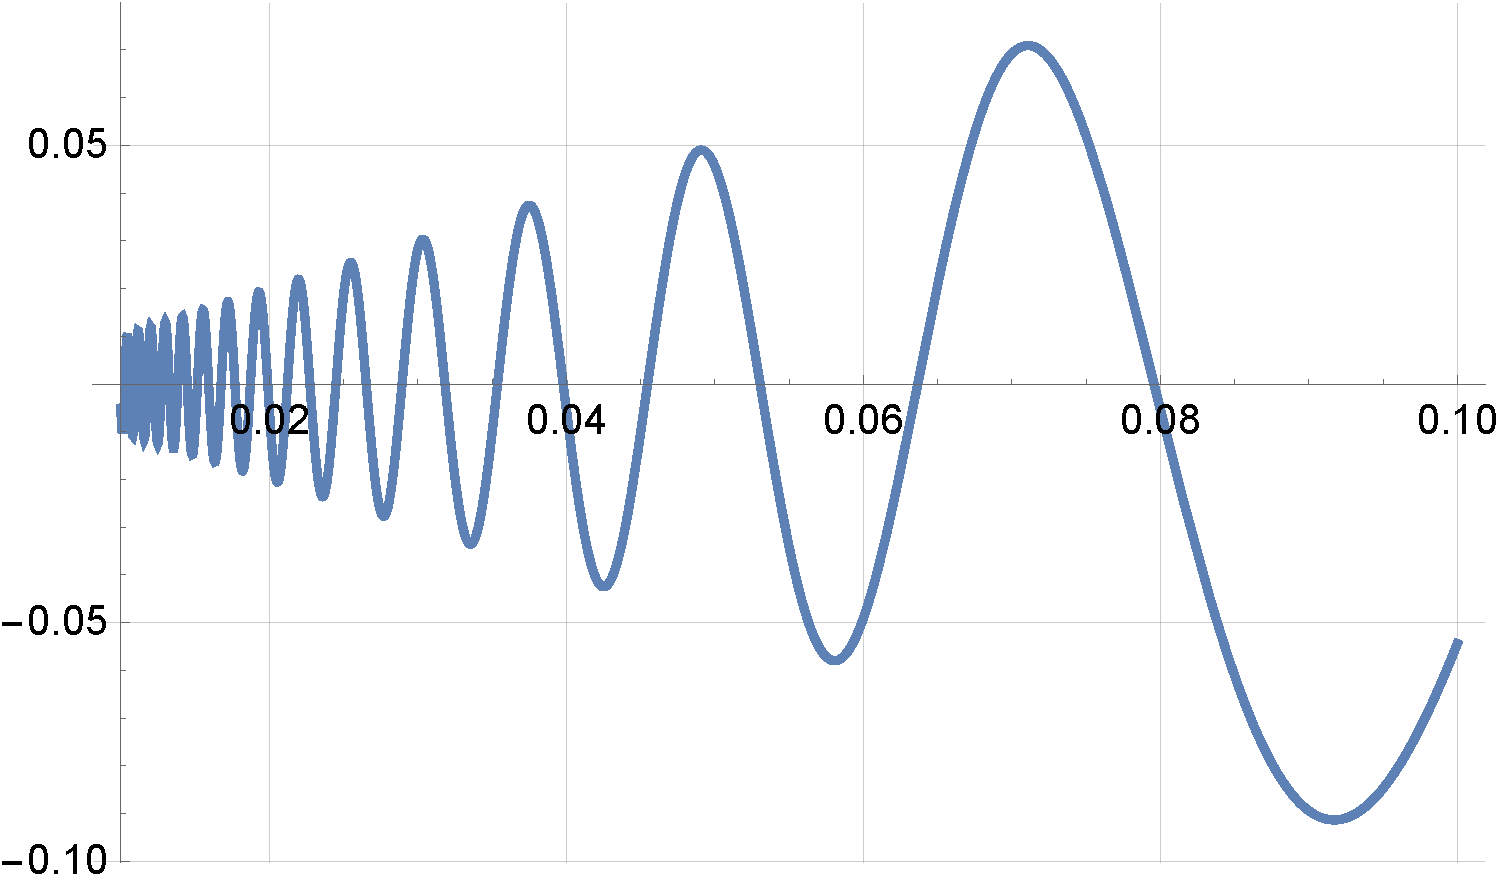
\includegraphics[width=0.5\textwidth]{../Figures/func2.pdf}
    \caption{Function 2}
    \label{fig:func2}
\end{figure}

For this function, the analytical solution for the integral is given by Eq. \eqref{eq:func2_integral}
\begin{equation}
    \label{eq:func2_integral}
    \int x\sin\left(\frac{1}{x}\right) ~dx = \frac{x}{2}\cos\left(\frac{1}{x}\right) + \frac{x^2}{2}\sin\left(\frac{1}{x}\right) + \frac{1}{2}\text{Si}\left(\frac{1}{x}\right),
\end{equation}
in which Si is the Sine Integral Function, defined by Eq. \eqref{eq:sine_integral}
\begin{equation}
    \label{eq:sine_integral}
    \text{Si}(z) = \int_{0}^{z} \frac{\sin(t)}{t} ~dt.
\end{equation}
Eq. \eqref{eq:sine_integral} can be approximated by the Pad\'e approximants of the convergent Taylor Series, available in \href{https://en.wikipedia.org/wiki/Trigonometric_integral#Asymptotic_series_(for_large_argument)}{here}.

\subsection{Function 3}
Finally, Function 3 is given by Eq. \eqref{eq:func3} and Fig. \ref{fig:func3} shows its behaviour
\begin{equation}
    \label{eq:func3}
    f(x) = 
    \begin{cases}
        2x + 5 \quad &0 \leq x \leq 1/\pi \\
        \frac{-5\pi^2(x^2-2x-5) + 10\pi x + 2x}{1 + 5\pi^2} \quad &1/\pi \leq x \leq 2/\pi\\
        2\sin(2x) + \frac{4+20\pi^2+25\pi^3}{\pi + 5\pi^3} - 2\sin\left(\frac{4}{\pi}\right) \quad &2/\pi \leq x \leq 8/\pi
    \end{cases}.
\end{equation}
\begin{figure}[H]
    \centering
    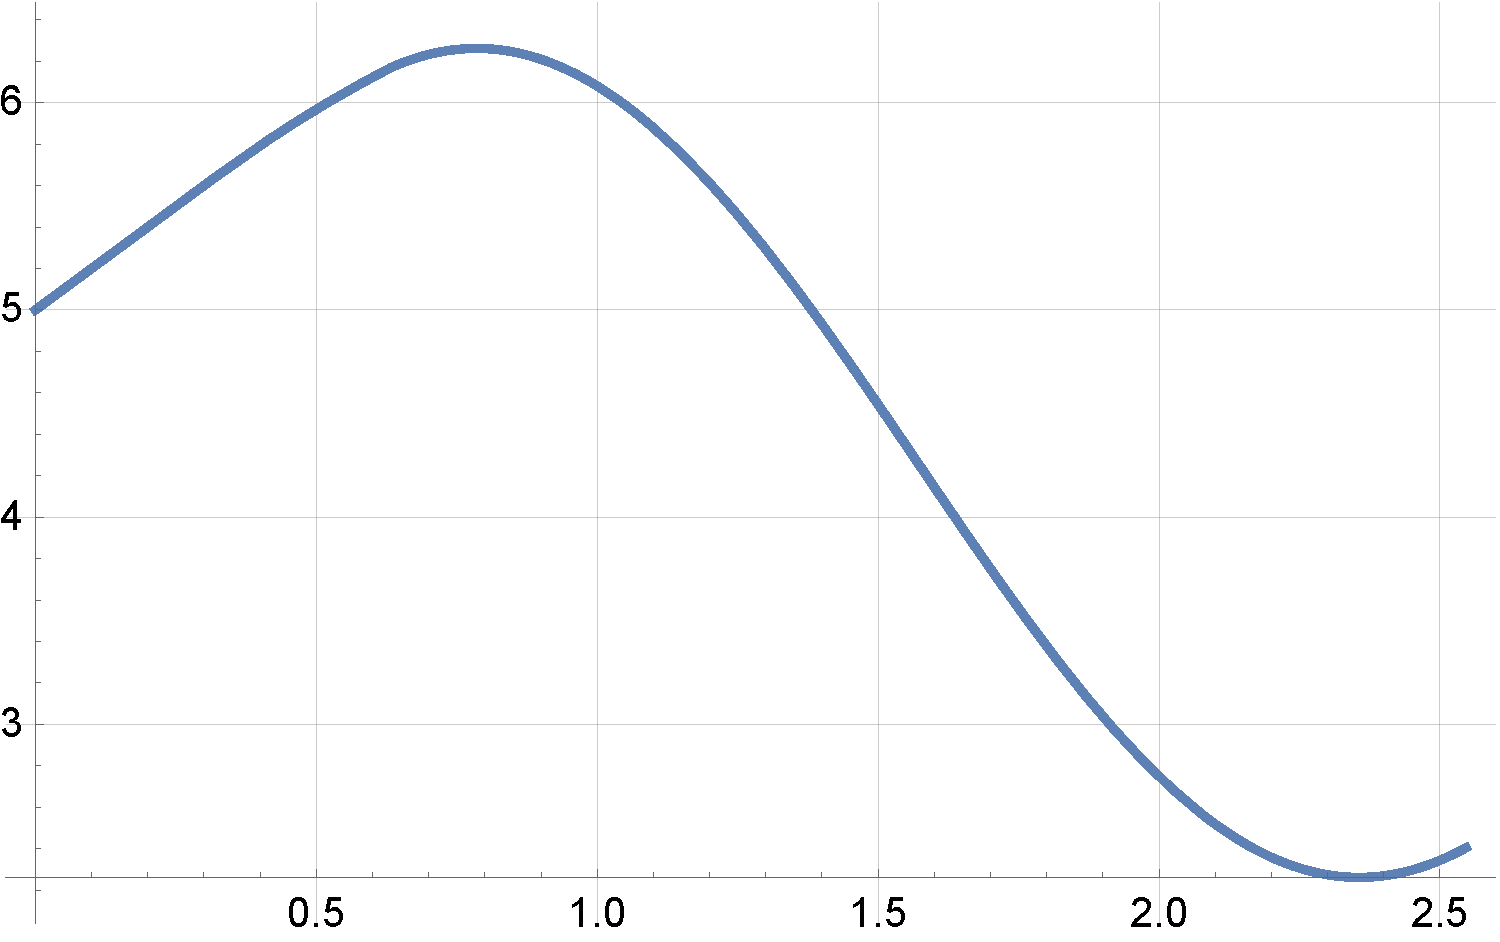
\includegraphics[width=0.5\textwidth]{../Figures/func3.pdf}
    \caption{Function 3}
    \label{fig:func3}
\end{figure}

Since the antiderivative of this function is a piecewise function, the analytical solution for the integral is given by parts as well (see Eq. \eqref{eq:func3_integral})
\begin{equation}
    \label{eq:func3_integral}
    \int f(x) ~dx = 
    \begin{cases}
        x^2 + 5x \quad &0 \leq x \leq 1/\pi \\
        \frac{25\pi^2x + x^2 + 5\pi x^2 + 5\pi^2x^2 - \frac{5\pi^2x^3}{3}}{1+5\pi^2} \quad &1/\pi \leq x \leq 2/\pi\\
        \frac{(4+20\pi^2+25\pi^3)x}{\pi + 5\pi^3} -\cos(2x) - 2x\sin\left(\frac{4}{\pi}\right) \quad &2/\pi \leq x \leq 8/\pi
    \end{cases}.
\end{equation} 